\documentclass[12pt,a4paper]{article}
% 文档类:12pt字体,A4纸张,文章类型
\usepackage[margin=1in]{geometry}
% 几何包:设置1英寸边距
\usepackage{graphicx}
% 图形包:插入图片
\usepackage{amsmath}
% AMS数学包:数学公式
\usepackage{amssymb}
% AMS符号包:数学符号
\usepackage{newtxtext,newtxmath} % Times New Roman 字体
% New TX字体包:Times New Roman字体
\usepackage{setspace} % 行距设置
% Setspace包:行距设置
\usepackage{siunitx}
% SI单位包:科学单位
\usepackage[hidelinks]{hyperref} % 去除目录/链接红框
\usepackage[backend=biber, style=ieee]{biblatex}
\addbibresource{references.bib}
% Hyperref包:超链接,隐藏链接边框
\usepackage{enumitem}
% Enumitem包:列表项
\usepackage{float}
% Float包:浮动环境
\usepackage{subcaption}
% Subcaption包:子标题
\usepackage{tikz}
% TikZ包:绘制图形
\usetikzlibrary{shapes,arrows,positioning,fit,backgrounds}


% 设置页面格式:1英寸边距,1.5倍行距,12点Times New Roman字体
\geometry{margin=1in}
\onehalfspacing
\setlength{\parindent}{0pt}
\setlength{\parskip}{6pt}

\title{\textbf{EE5112: Human Robot Interaction\\Project 1: Dialogue System and LLM Platform Development}}
% 标题:EE5112:人机交互\\项目1:对话系统和LLM平台开发
\author{Group 7\\
Niu Mu (Matriculation Number)\\
Wu Zining (A0294373W)\\
Zhao Jinqiu (Matriculation Number)}
\date{\today}
% 日期:今天

\begin{document}
% 文档开始

\maketitle
% 生成标题页

% 标题页
% Title page with group information and course details

\newpage
% 新页

\tableofcontents
% 生成目录

\newpage
% 新页

% 目录
% Table of contents

\section{Abstract}
% 摘要

% 摘要部分 - 简要概述项目目标、方法、主要发现和结论
% Abstract section - Brief overview of project objectives, methods, key findings and conclusions

[Placeholder for abstract content - 150-250 words]
% [摘要内容占位符 - 150-250字]

% 关键词
% Keywords
\textbf{Keywords:} Dialogue System, LLM, Human-Robot Interaction, Natural Language Processing, TensorFlow
% 关键词:对话系统,LLM,人机交互,自然语言处理,TensorFlow

\section{Introduction}
% 引言

% 引言部分 - 介绍对话系统和LLM的背景,项目目标和意义
% Introduction section - Background of dialogue systems and LLMs, project objectives and significance

\subsection{Background}
% 背景

% 背景介绍 - 对话系统在人机交互中的重要性
% Background introduction - Importance of dialogue systems in human-robot interaction

[Placeholder for background content]
% [背景内容占位符]

\subsection{Project Objectives}
% 项目目标

% 项目目标 - 基于课程要求的具体目标
% Project objectives - Specific objectives based on course requirements

The main objectives of this project are:
% 本项目的主要目标是:
\begin{enumerate}
    \item To familiarize with the process of developing a dialogue system
    % 熟悉对话系统开发过程
    \item To familiarize with the working environment and Python packages
    % 熟悉工作环境和Python包
    \item To familiarize with popular platforms such as TensorFlow
    % 熟悉TensorFlow等流行平台
    \item To familiarize with popular open source LLMs (Llama, GLM, etc.)
    % 熟悉Llama、GLM等流行开源LLM
    \item To develop a dialogue system and local LLM platform
    % 开发对话系统和本地LLM平台
    \item To familiarize with LLM evaluation procedures
    % 熟悉LLM评估程序
    \item To provide practical experience in problem-finding and problem-solving
    % 提供问题发现和解决的实践经验
\end{enumerate}


% Task1 
\section{Task 1: Develop the Dialogue Systems according to aspiration/interest.}

% Task2
\section{Task 2: Develop Local Dialogue Systems by Using Open-Source LLMs}

\subsection{Literature Review on Different Categories of LLMs}
% 不同类型LLM的文献综述

Large Language Models (LLMs) can be broadly categorized into three main architectures based on their use of the transformer mechanism \cite{vaswani2017attention}: Encoder-Decoder, Encoder-Only, and Decoder-Only. Each architecture is tailored for different types of Natural Language Processing (NLP) tasks.
% 大型语言模型(LLM)可根据其对Transformer机制的使用情况\cite{vaswani2017attention},大致分为三种主要架构:编码器-解码器、仅编码器和仅解码器。每种架构都针对不同类型的自然语言处理(NLP)任务进行了优化。

\begin{itemize}
    \item \textbf{Encoder-Decoder models}, such as T5 \cite{raffel2020exploring} and BART \cite{lewis2019bart}, utilize both a bidirectional encoder to process the input text and an autoregressive decoder to generate output. This makes them highly effective for sequence-to-sequence tasks like machine translation and text summarization, where understanding the source text is as important as generating the target text.
    % \textbf{编码器-解码器模型},如T5 \cite{raffel2020exploring}和BART \cite{lewis2019bart},同时使用双向编码器处理输入文本和自回归解码器生成输出。这使得它们在机器翻译和文本摘要等序列到序列任务中非常有效,因为在这些任务中,理解源文本与生成目标文本同样重要。
    \item \textbf{Encoder-Only models}, like BERT \cite{devlin2018bert} and RoBERTa \cite{liu2019roberta}, use only the bidirectional encoder. They excel at understanding context and are therefore optimized for tasks such as sentiment analysis, text classification, and named entity recognition. However, they are not inherently suited for text generation.
    % \textbf{仅编码器模型},如BERT \cite{devlin2018bert}和RoBERTa \cite{liu2019roberta},仅使用双向编码器。它们擅长理解上下文,因此针对情感分析、文本分类和命名实体识别等任务进行了优化。然而,它们本身不适合文本生成。
    \item \textbf{Decoder-Only models}, including the GPT series \cite{radford2018improving} and LLaMA \cite{touvron2023llama}, employ a unidirectional (causal) decoder. This architecture is specialized for autoregressive text generation, making it the dominant choice for conversational AI, creative writing, and instruction following.
    % \textbf{仅解码器模型},包括GPT系列 \cite{radford2018improving}和LLaMA \cite{touvron2023llama},采用单向(因果)解码器。该架构专门用于自回归文本生成,使其成为对话AI、创意写作和指令遵循的主流选择。
\end{itemize}

The key differences, performance trade-offs, and typical applications of these architectures are summarized in Table~\ref{tab:llm_comparison}. Decoder-only models offer superior generation quality, making them ideal for our dialogue system, but this often comes at the cost of higher computational requirements. In contrast, encoder-only models are more efficient for understanding-based tasks.
% 这些架构的关键差异、性能权衡和典型应用总结在表~\ref{tab:llm_comparison}中。仅解码器模型提供卓越的生成质量,使其成为我们对话系统的理想选择,但这通常以更高的计算要求为代价。相比之下,仅编码器模型在基于理解的任务上更高效。

\begin{table}[H]
\centering
\caption{Comparison of LLM Architecture Types}
% LLM架构类型比较
\label{tab:llm_comparison}
\begin{tabular}{|l|l|l|l|}
\hline
\textbf{Aspect} & \textbf{Encoder-Decoder} & \textbf{Encoder-Only} & \textbf{Decoder-Only} \\
% 方面 & 编码器-解码器 & 仅编码器 & 仅解码器
\hline
Primary Use & Seq2Seq tasks & Understanding tasks & Generation tasks \\
% 主要用途 & Seq2Seq任务 & 理解任务 & 生成任务
\hline
Attention & Bidirectional + Causal & Bidirectional & Causal \\
% 注意力机制 & 双向 + 因果 & 双向 & 因果
\hline
Task Flexibility & High & Medium & High \\
% 任务灵活性 & 高 & 中等 & 高
\hline
Representative Models & T5, BART & BERT, RoBERTa & GPT, LLaMA \\
% 代表性模型 & T5, BART & BERT, RoBERTa & GPT, LLaMA
\hline
\end{tabular}
\end{table}

Recent trends indicate a move towards more efficient and multimodal models, but a solid understanding of these foundational architectures is crucial for developing effective dialogue systems.
% 最近的趋势表明,模型正朝着更高效和多模态的方向发展,但对这些基础架构的深入理解对于开发有效的对话系统至关重要。

% 对不同LLM架构的全面理解为在对话系统和本地LLM平台中选择适当模型提供了基础。




% Task 2.2
\subsection{Local LLM Platform Implementation}

We deploy a compact local dialogue stack around the quantized \texttt{Llama-3.2-3B-Instruct-Q4\_K\_M.gguf} checkpoint to provide offline interaction without sacrificing responsiveness.
% 部署基于量化 Llama-3.2-3B-Instruct-Q4_K_M.gguf 的轻量本地对话栈,实现离线交互并保持响应速度

\noindent\textbf{Architecture.} \texttt{llm\_platform.py} wraps \texttt{llama-cpp-python} for model loading and inference, while \texttt{dialogue\_system.py} manages the chat loop, prompt templating, streaming output, and defensive error handling. The separation keeps model plumbing isolated from user interaction logic.
% 架构层面将模型加载推理与对话管理解耦,llm_platform.py 负责底层推理,dialogue_system.py 负责交互与容错

\noindent\textbf{Inference pipeline.} Configuration values expose only the essentials: a 4,096-token context window, generation controls (temperature and maximum new tokens), and an optional GPU layer count for acceleration. Switching between CPU and CUDA execution is done in \texttt{config.json} without touching the code base.
% 推理流程仅暴露上下文长度、采样控制和 GPU 层数等核心参数,可在 config.json 中无缝切换 CPU/GPU

\noindent\textbf{User experience and persistence.} The terminal interface streams tokens as they are produced, retains up to six dialogue turns, supports maintenance commands (\texttt{exit}/\texttt{clear}/\texttt{stats}), and records each session as ISO8601-stamped JSON under \texttt{conversations/} for later auditing.
% 终端界面支持流式输出、保留最多六轮上下文,提供退出/清除/统计命令,并以 ISO8601 时间戳保存会话记录

\noindent\textbf{Portability.} The same stack runs on laptops or desktop GPUs, making it suitable for privacy-sensitive deployments and quick benchmarking. Figure~\ref{fig:llama_cpu_chat} illustrates the interface operating in CPU mode.
% 该方案可在笔记本或桌面 GPU 上部署,兼顾隐私场景与快速评测,图~\ref{fig:llama_cpu_chat} 展示其 CPU 模式界面

\begin{figure}[H]
    \centering
    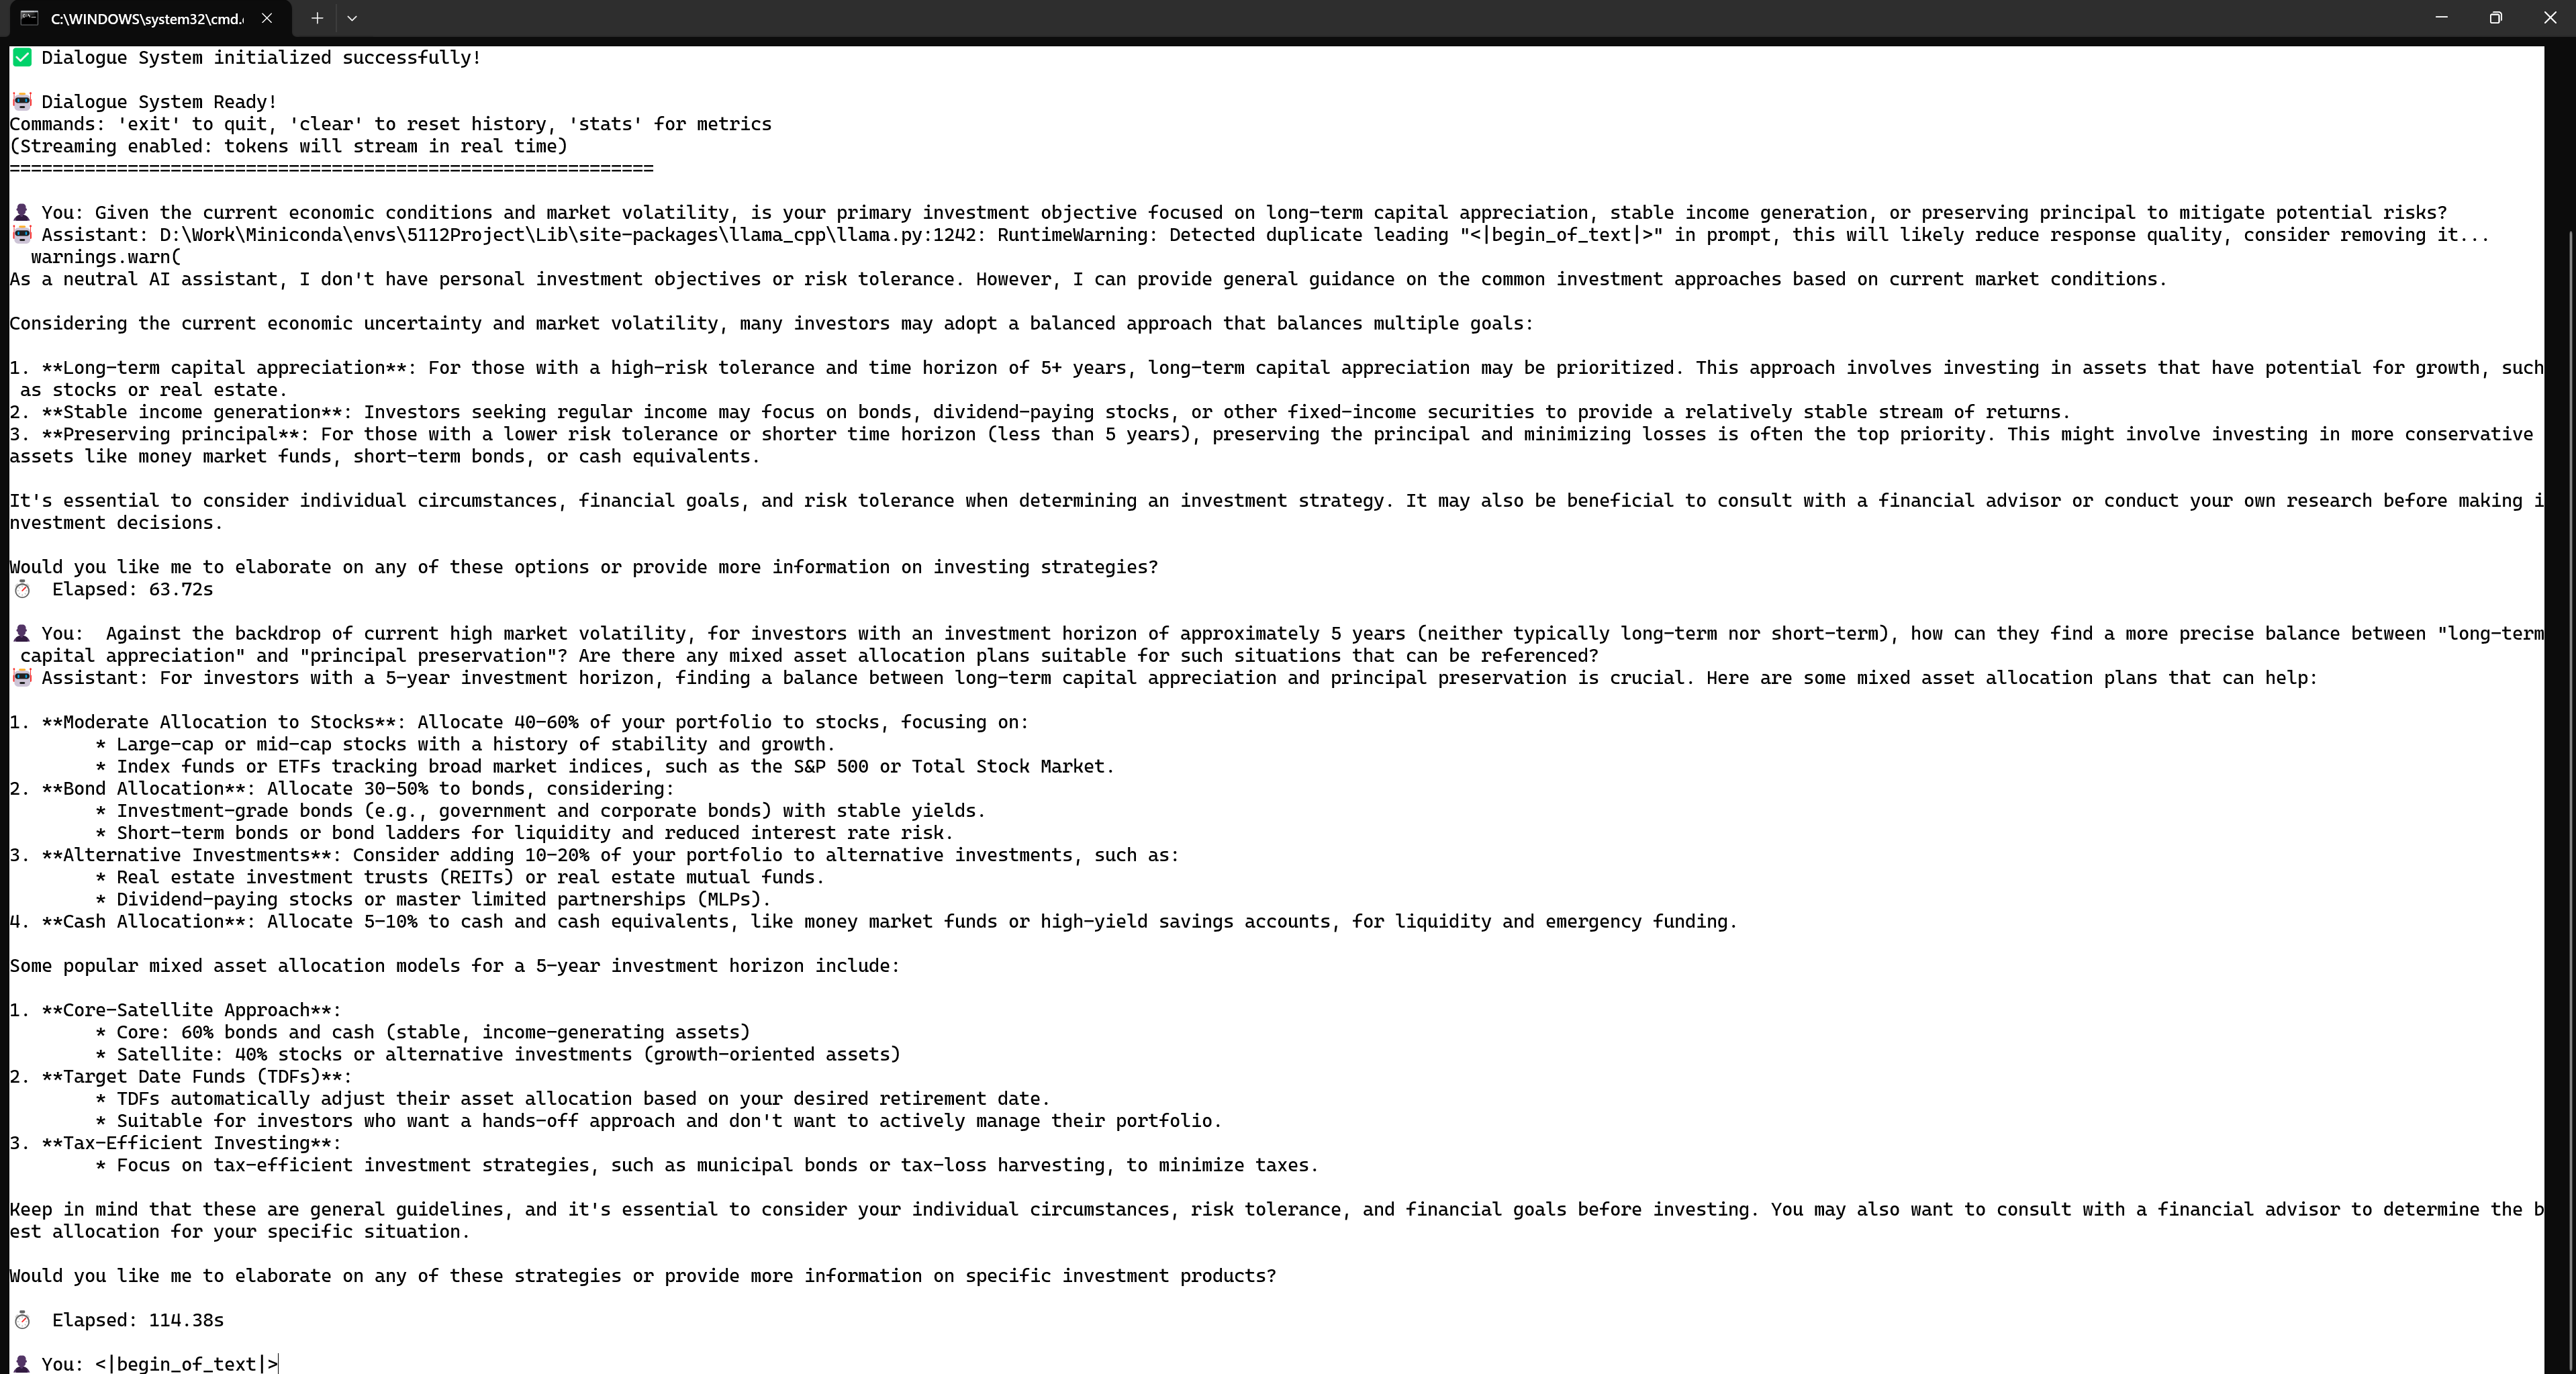
\includegraphics[width=0.95\linewidth]{Figures/llama对话.png}
    \caption{Terminal-based dialogue interface showing multi-turn conversation capabilities}
    \label{fig:llama_cpu_chat}
\end{figure}


\subsection{Challenges in Deployment}

Our initial deployment relied on the Hugging Face Transformers stack with the full Llama-3.1-8B-Instruct checkpoint. Despite enabling flash attention and trimming sequence length, the 16~GiB RTX~5080 could not accommodate FP16 weights together with KV caches; each inference exhausted memory and crashed the dialogue loop with CUDA out-of-memory errors.
% 首轮部署尝试使用 Hugging Face Transformers 加载 Llama-3.1-8B-Instruct。即便启用 flash attention 并缩短序列长度,16~GiB RTX~5080 仍无法同时容纳 FP16 权重与 KV 缓存,推理过程中不断触发 CUDA OOM。

We then switched the same checkpoint to vLLM, hoping paged attention would ease the pressure. However, Windows-specific driver and wheel mismatches caused the runtime to halt during initialization because `cublas` dependencies failed to load.
% 之后将模型迁移到 vLLM,希望 paged attention 可以缓解显存压力,但在 Windows 环境下因驱动与 Python 轮子版本不匹配,cublas 依赖加载失败,系统在初始化阶段即终止。

Finally, we quantized Llama-3.2-3B to Q4\_K\_M and served it through llama.cpp. After reinstalling a CUDA-enabled `llama-cpp-python` wheel and exposing the NVIDIA runtime DLLs, the GPU backend became stable and remained well within memory limits, so this setup was adopted for the project.
% 最终将 Llama-3.2-3B 量化为 Q4\_K\_M,并通过 llama.cpp 推理;重新安装支持 CUDA 的 `llama-cpp-python` 并补齐 NVIDIA 运行库后,GPU 推理稳定且显存占用可控,因此成为项目最终采用的方案。



\subsection{Performance Comparison: CPU vs GPU Deployment}
% 性能比较:CPU 与 GPU 部署

To quantify the benefit of the dedicated GPU pipeline, we benchmarked identical prompts (\textit{"hello"} and \textit{"Who are you?"}) on both deployment targets using the same quantized \texttt{Llama-3.2-3B-Instruct-Q4\_K\_M.gguf} model and configuration. Timing was captured end-to-end from user input to the final token, with streaming enabled in both runs. The GPU test was executed on an RTX 5080 16GB with cuBLAS acceleration, whereas the CPU baseline was collected on the same workstation with GPU offloading disabled.
% 为量化 GPU 管线带来的收益,我们在 CPU 与 GPU 上使用相同提示词和同一量化模型进行基准测试,记录从输入到生成完成的端到端耗时。

\begin{table}[H]
    \centering
    \caption{Inference latency comparison between CPU and GPU backends}
    % CPU 与 GPU 推理延迟比较
    \label{tab:cpu_gpu_latency}
    \begin{tabular}{|l|c|c|c|}
        \hline
        	extbf{Prompt} & \textbf{CPU latency (s)} & \textbf{GPU latency (s)} & \textbf{Speedup} \\
        % 提示词 & CPU 延迟 & GPU 延迟 & 加速比
        \hline
        hello & 4.90 & 0.595 & 8.2\texttimes{} \\
        Who are you? & 22.40 & 1.35 & 16.6\texttimes{} \\
        \hline
    \end{tabular}
\end{table}

Across both prompts, the GPU path delivers dramatic performance improvements, achieving 8.2× speedup for short prompts and 16.6× speedup for longer responses while preserving output quality. The substantial reduction primarily stems from mapping transformer layers onto CUDA kernels (\texttt{n\_gpu\_layers = -1}) via \texttt{llama-cpp-python} with \texttt{LLAMA\_CUBLAS=1}, eliminating the CPU bottleneck observed in the baseline. The sub-second response times significantly improve conversational fluidity because streamed tokens begin appearing almost immediately, keeping the user engaged.
% GPU 方案实现了显著的性能提升,短提示词加速 8.2 倍,长回复加速 16.6 倍,主要得益于使用 cuBLAS 将 transformer 层映射到 GPU,从而消除 CPU 瓶颈。

Figure~\ref{fig:llama_cpu_chat} shows the slower CPU baseline, while Figure~\ref{fig:llama_gpu_chat} captures the accelerated GPU session that produced the timings in Table~\ref{tab:cpu_gpu_latency}.
% 图~\ref{fig:llama_cpu_chat} 展示 CPU 基线,图~\ref{fig:llama_gpu_chat} 对应 GPU 加速会话。

\begin{figure}[H]
    \centering
    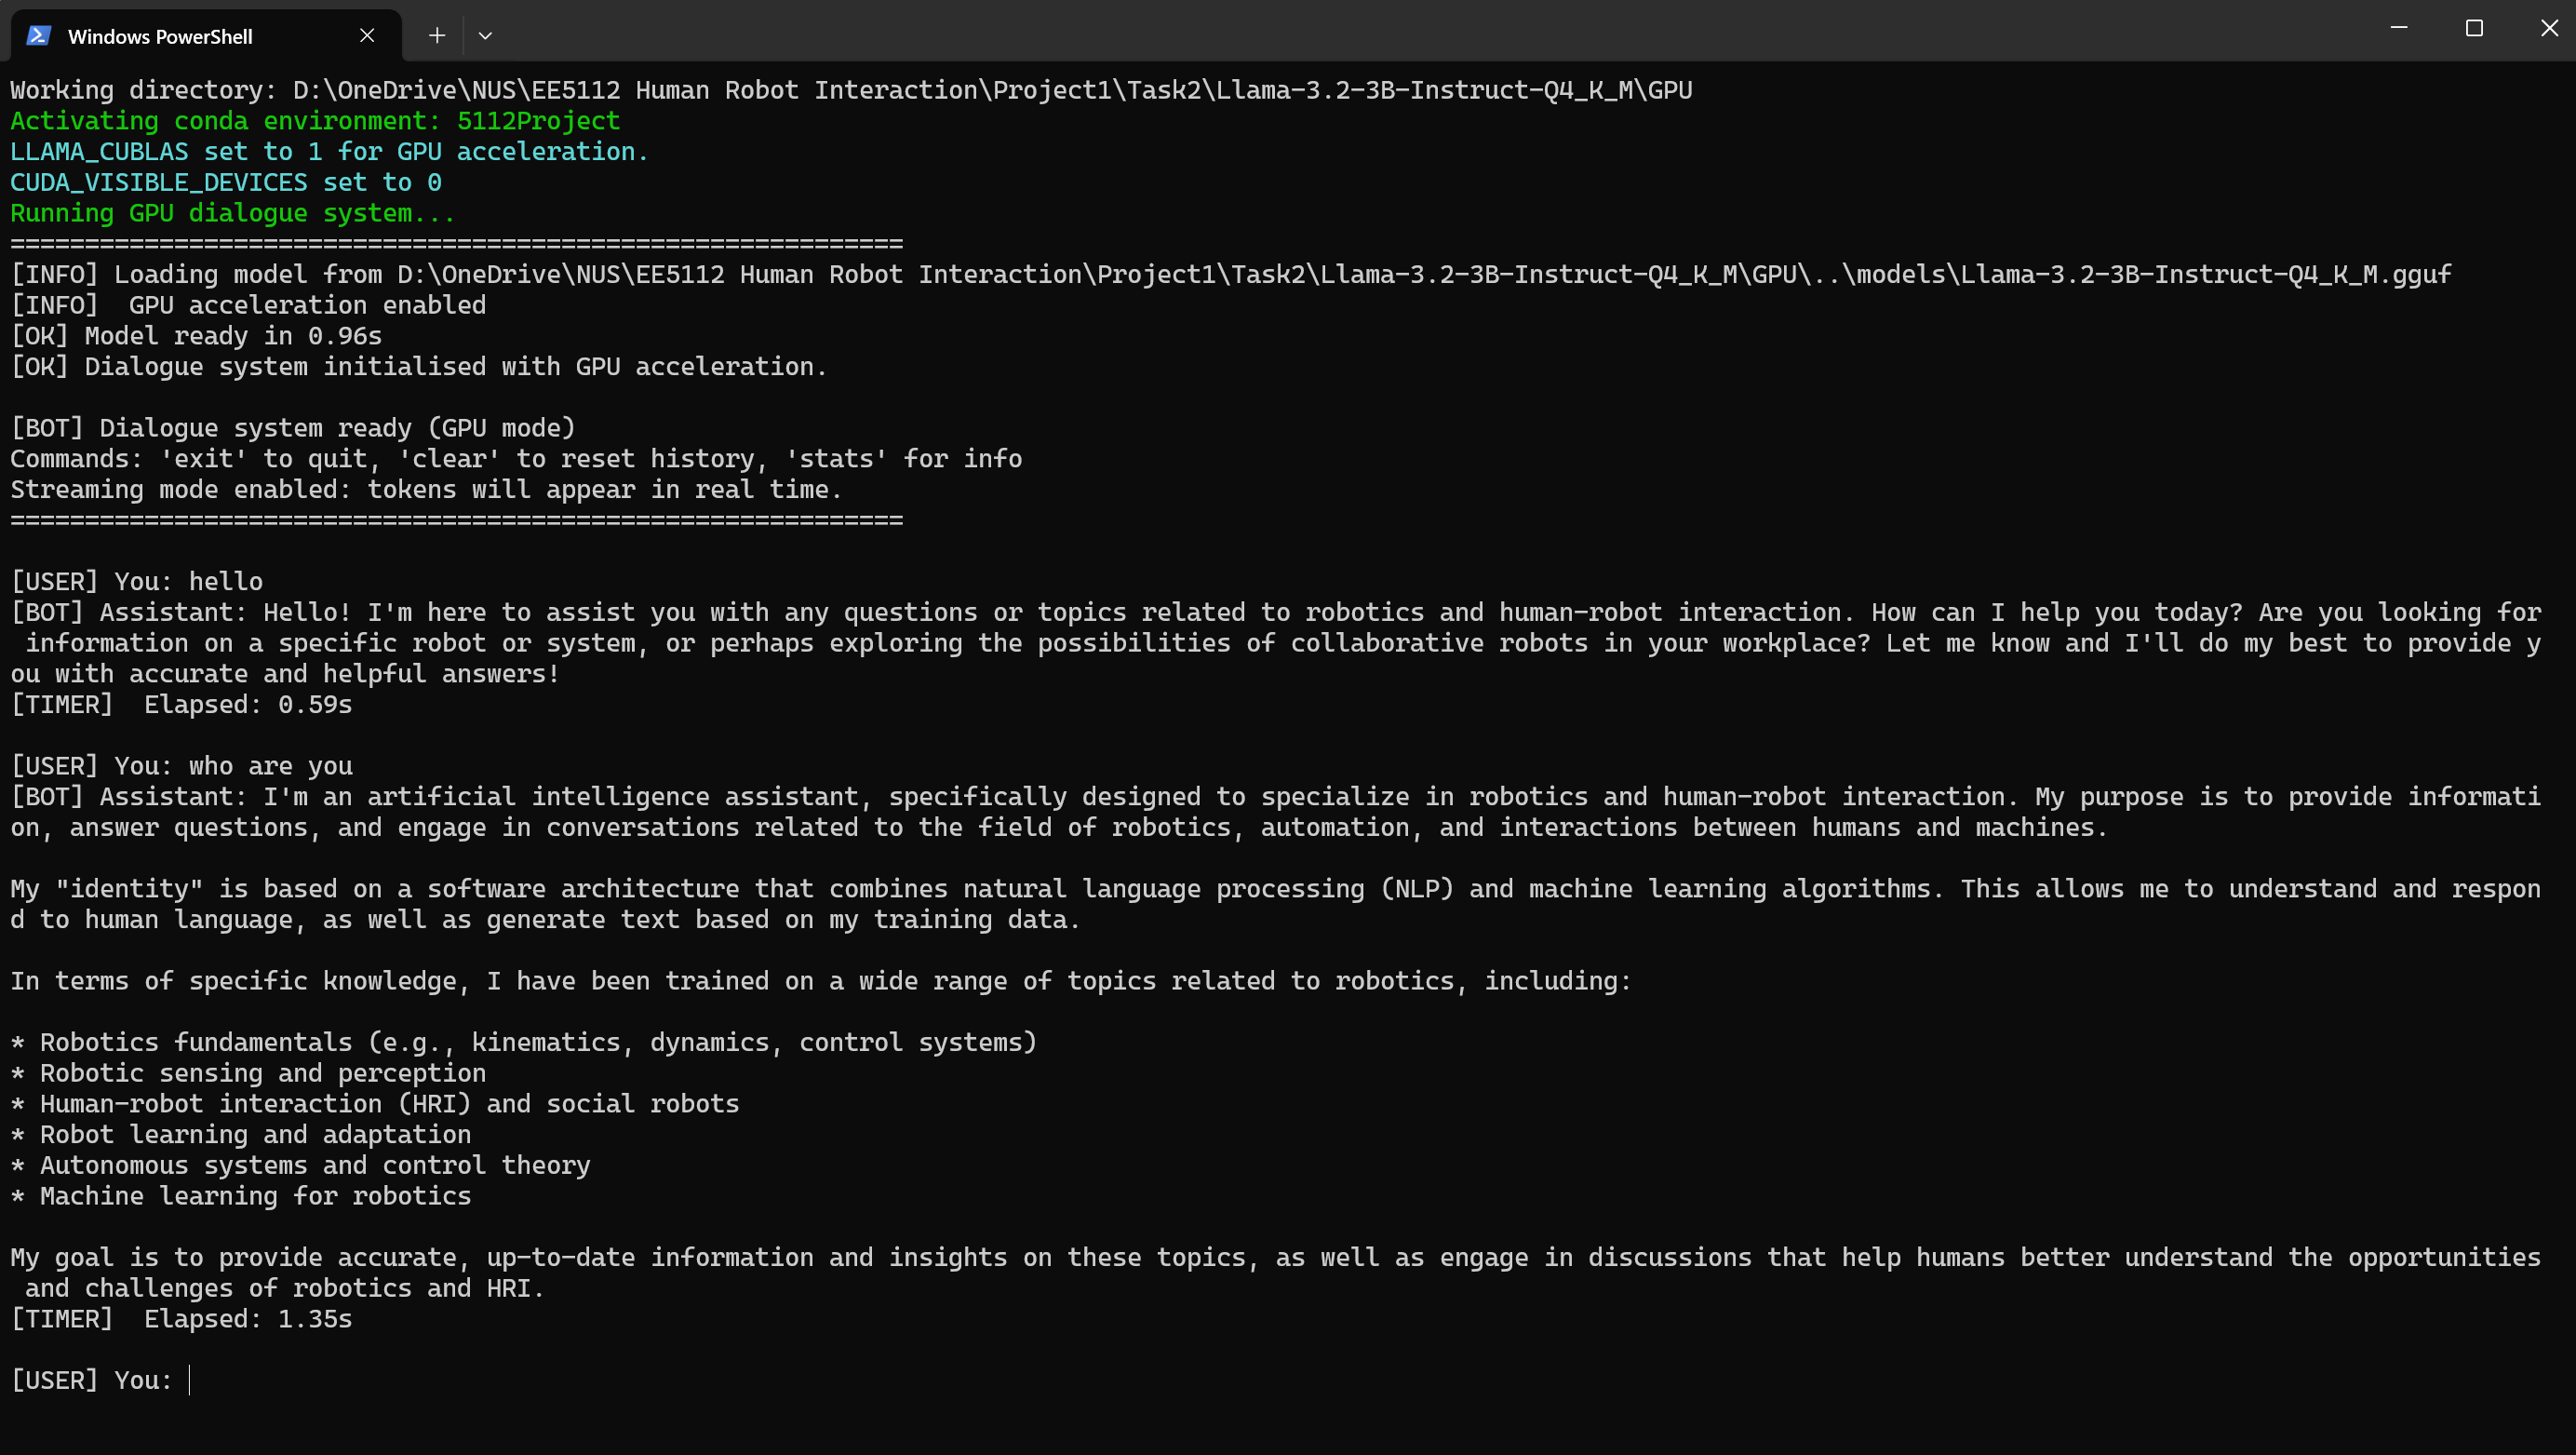
\includegraphics[width=1\linewidth]{Figures/llamaGPU.png}
    \caption{Streaming dialogue captured during the GPU benchmark run.}
    % GPU 基准运行时捕获的流式对话截图
    \label{fig:llama_gpu_chat}
\end{figure}





\subsection{Comparison of Different Pretrained Models}
% 不同预训练模型的比较

To evaluate the reasoning capabilities and response quality of different model variants, we conducted a comparative analysis between Llama-3.1-8B-Instruct and Llama-3.2-3B-Instruct using a logical reasoning task. The test involved a constraint satisfaction problem requiring systematic analysis and deductive reasoning.
% 为评估不同模型变体的推理能力和响应质量,我们使用逻辑推理任务对 Llama-3.1-8B-Instruct 和 Llama-3.2-3B-Instruct 进行了比较分析。

\subsubsection{Logical Reasoning Test}
% 逻辑推理测试

The test prompt presented a constraint satisfaction problem: \textit{"Logic reasoning: A not 1st, C not last, B not 1st or last, what is ranking?"} This requires the model to systematically analyze multiple constraints and derive a valid solution through logical deduction.
% 测试提示提出了一个约束满足问题,要求模型系统性地分析多个约束条件并通过逻辑推演得出有效解。

\begin{figure}[H]
    \centering
    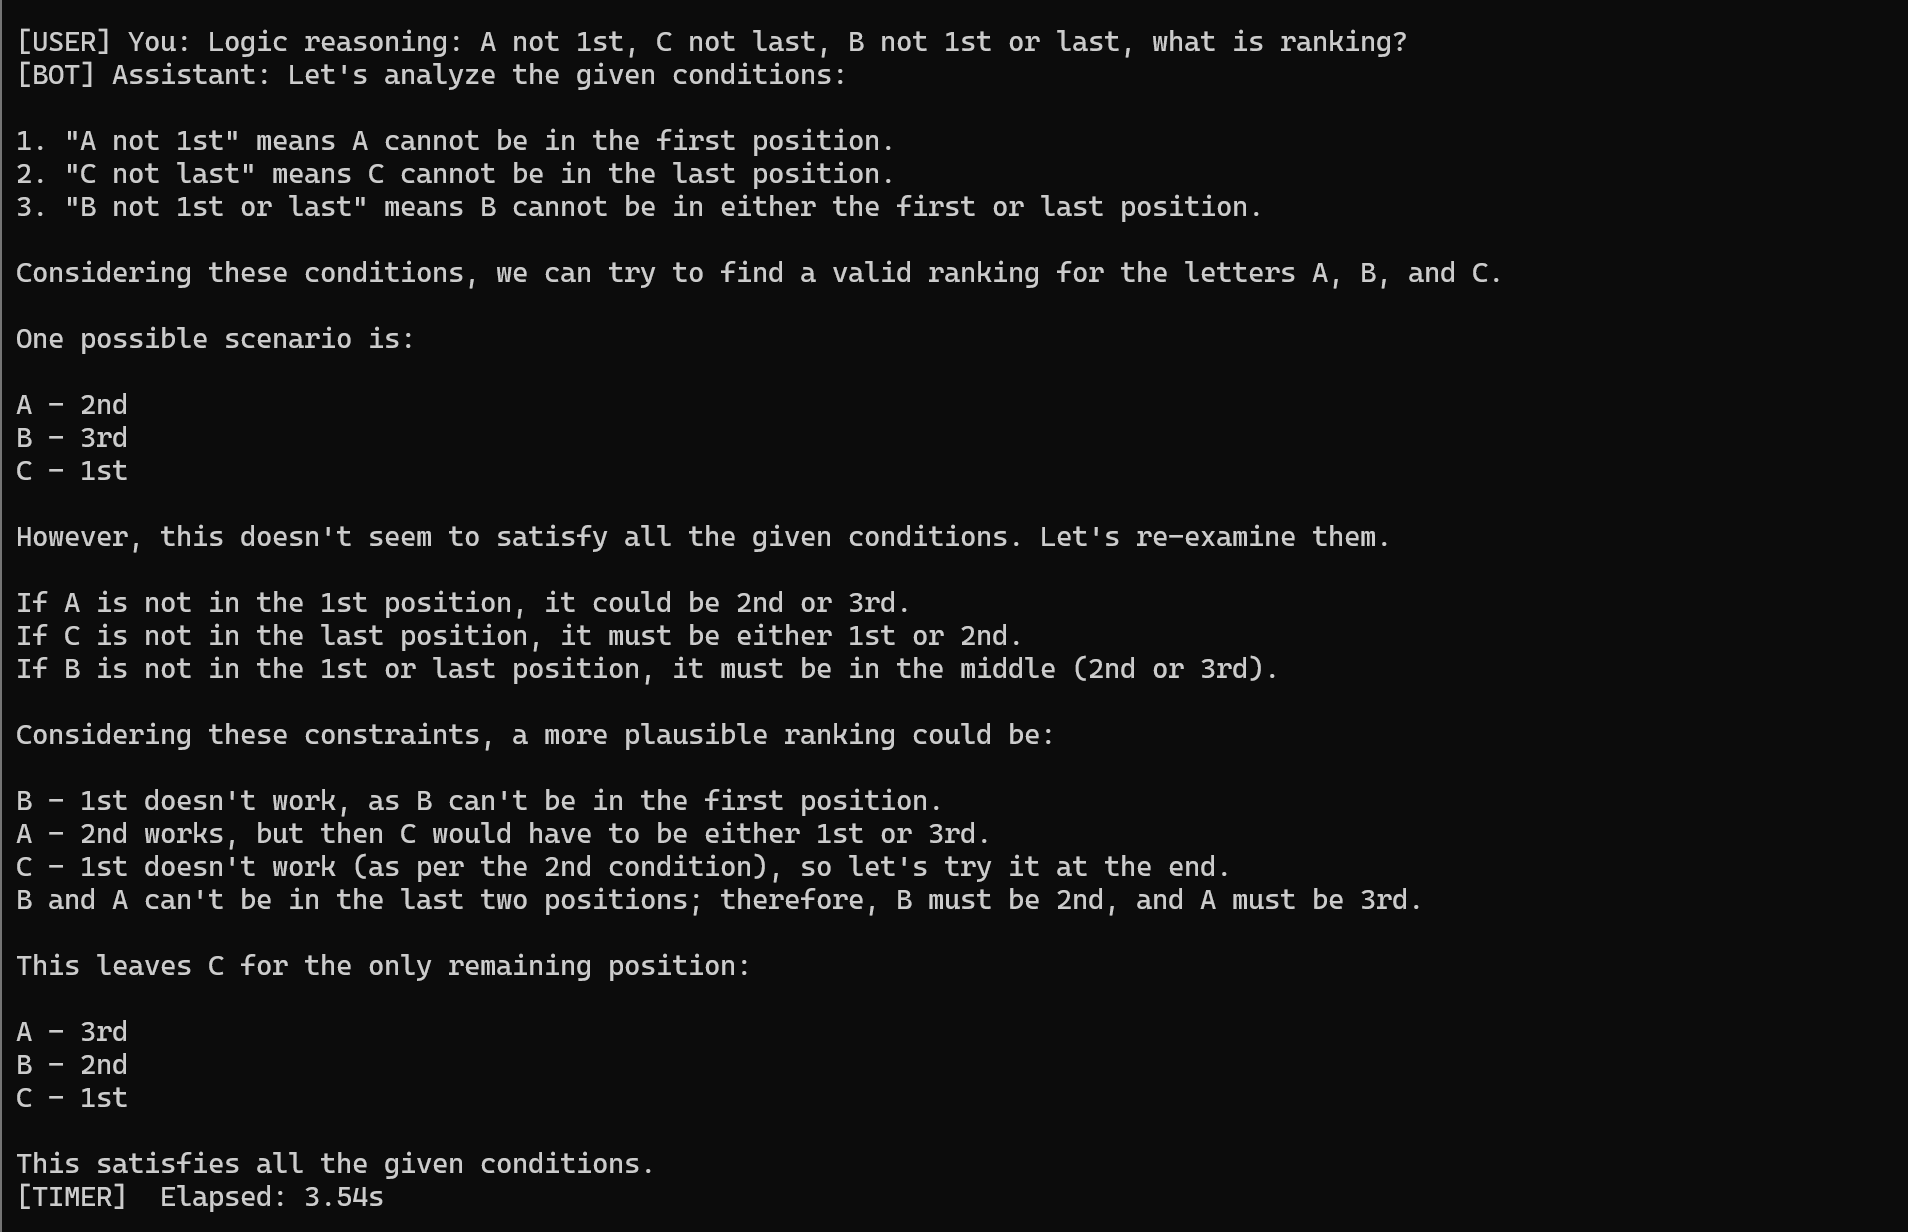
\includegraphics[width=0.95\linewidth]{Figures/3.1-8B ans.png}
    \caption{Llama-3.1-8B-Instruct response showing systematic logical analysis}
    \label{fig:llama31_reasoning}
\end{figure}

\begin{figure}[H]
    \centering
    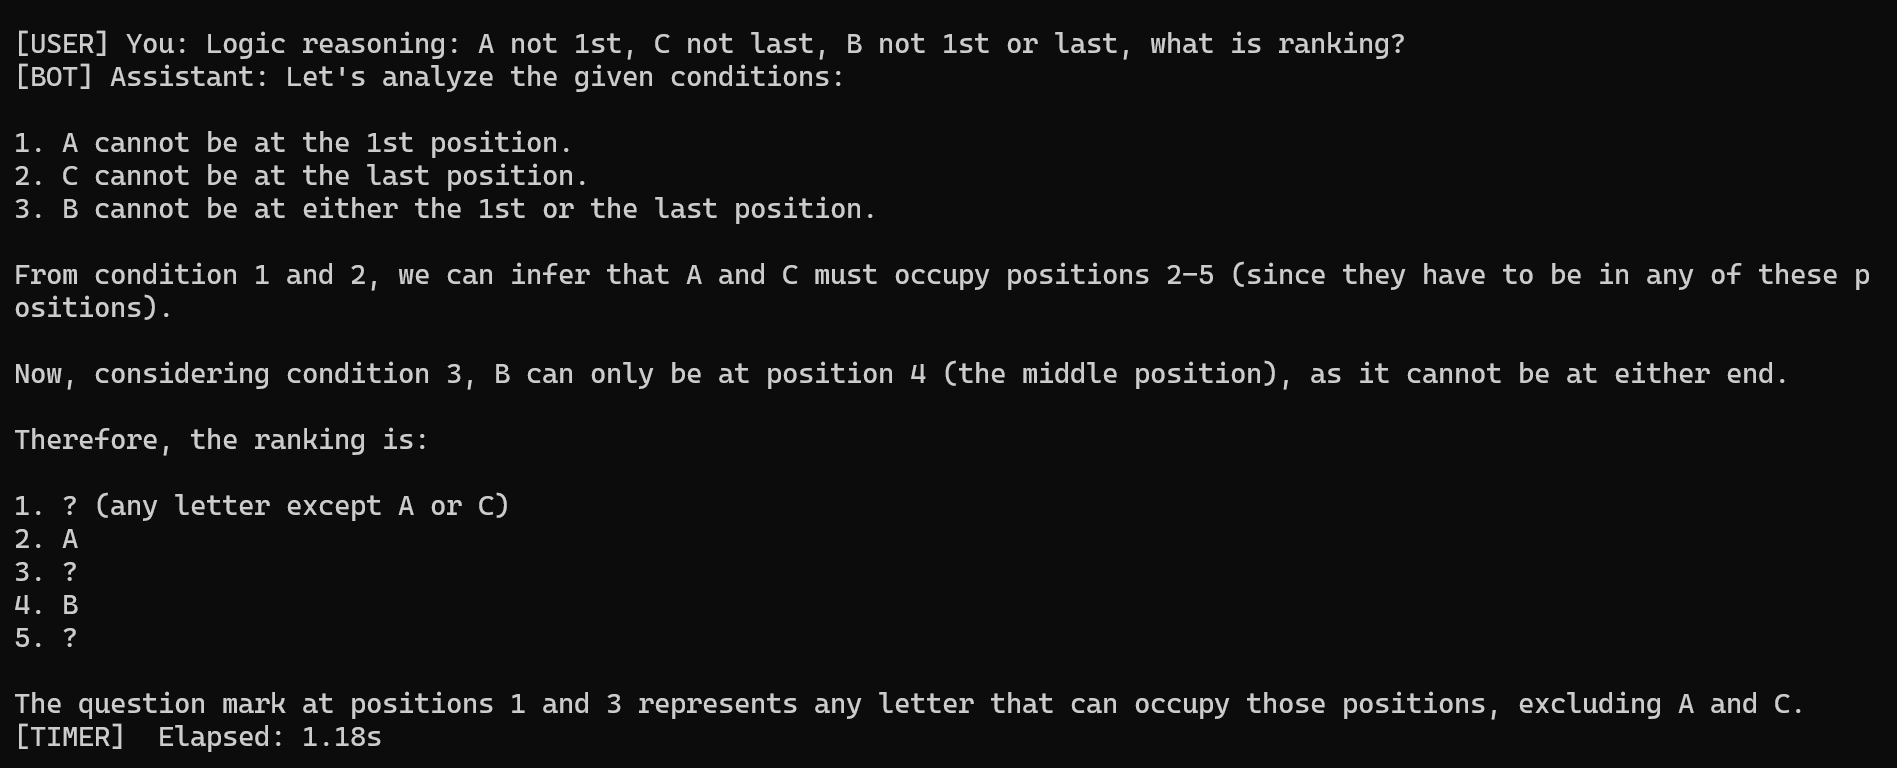
\includegraphics[width=0.95\linewidth]{Figures/3.2-3B ans.png}
    \caption{Llama-3.2-3B-Instruct response demonstrating structured problem-solving}
    \label{fig:llama32_reasoning}
\end{figure}

\subsubsection{Performance Analysis}
% 性能分析

\textbf{Llama-3.1-8B-Instruct} demonstrated comprehensive analytical capabilities with effective self-correction mechanisms. The model initially proposed an incorrect solution (A-2nd, B-3rd, C-1st) but recognized through systematic verification that this violated the constraints. It proceeded to re-examine the problem methodically, ultimately arriving at the correct ranking: A-3rd, B-2nd, C-1st. The response time was 3.64 seconds, reflecting the thorough analytical process including error detection and correction.
% Llama-3.1-8B-Instruct 展现了具有有效自我纠错机制的全面分析能力,响应时间为3.64秒,体现了包括错误检测和纠正在内的深入分析过程。

\textbf{Llama-3.2-3B-Instruct}, while demonstrating systematic constraint analysis, appears to have misinterpreted the problem scope. The model analyzed the constraints correctly but assumed a 5-position ranking system rather than recognizing this as a 3-element arrangement problem. Although its constraint analysis method was sound (identifying that A and C must occupy positions 2-5, and B must be in the middle), this fundamental misunderstanding of the problem structure led to an incomplete solution. The response time was 1.18 seconds.
% Llama-3.2-3B-Instruct 虽然展现了系统性的约束分析,但似乎误解了问题范围,假设了5位排名系统而非3元素排列问题,导致解答不完整。

\begin{table}[H]
\centering
\caption{Model comparison on logical reasoning task}
% 逻辑推理任务的模型比较
\label{tab:model_reasoning_comparison}
\begin{tabular}{|l|c|c|c|}
\hline
\textbf{Model} & \textbf{Response Time} & \textbf{Reasoning Style} & \textbf{Solution Quality} \\
% 模型 & 响应时间 & 推理风格 & 解答质量
\hline
Llama-3.1-8B & 3.64s & Self-correction & Complete \& Correct \\
% 自我纠错 & 完整正确
Llama-3.2-3B & 1.18s & Direct analysis & Incomplete \\
% 直接分析 & 不完整
\hline
\end{tabular}
\end{table}

This comparison reveals important insights about model capabilities: while the 3B model demonstrated faster processing and sound constraint analysis methodology, it failed to correctly interpret the problem scope. The 8B model, despite requiring more time, exhibited superior problem comprehension and self-correction abilities, ultimately delivering the complete and correct solution. This suggests that model size can significantly impact not just reasoning depth, but also problem interpretation accuracy in complex logical tasks.
% 这个比较揭示了模型能力的重要见解:虽然3B模型展现了更快的处理速度和合理的约束分析方法,但未能正确理解问题范围。8B模型尽管需要更多时间,但表现出更优的问题理解和自我纠错能力,最终提供了完整正确的解答。



% Task3
\section{Task 3: LLM Performance Evaluation}
% 任务3:LLM性能评估

[Placeholder for Task 3 content]
% [任务3内容占位符]

% Task4
\section{Task 4: GUI for Local LLM}
% 任务4:为本地LLM设计图形用户界面(GUI)

[Placeholder for Task 4 content]
% [任务4内容占位符]

% Task5
\section{Task 5: Exploring Multimodal Large Language Models (MLLMs)}
% 任务5:探索多模态大型语言模型(MLLMs)

Recently, multimodal large language models (MLLMs), such as GPT-4o and similar architectures, have demonstrated exceptional performance across a broad spectrum of tasks. These downstream tasks span interleaved conversations that integrate text, speech, and visuals, sophisticated image generation that understands context, and image question answering (IQA) capabilities. The advent of MLLMs marks a significant step forward in artificial intelligence, bridging multiple modalities to provide more interactive, context-aware outputs.
% 近年来,多模态大型语言模型(MLLMs),如GPT-4o等类似架构,在广泛的任务领域中展现了卓越的性能。这些下游任务涵盖了文本、语音和视觉的交错对话,理解上下文的复杂图像生成,以及图像问答(IQA)能力。MLLM的出现标志着人工智能的重大进步,连接多种模态以提供更具交互性、上下文感知的输出。

In this task, students are required to explore and understand the fundamentals of MLLMs, delving into their architecture, training processes, and practical applications. LLaVA (Large Language and Vision Assistant) serves as a practical example for this exploration. As outlined on their project page (https://llava-vl.github.io), LLaVA exemplifies how multimodal systems can be fine-tuned to enhance visual-language understanding, particularly in fields like image captioning, visual dialogue, and question answering.
% 在此任务中,学生需要探索和理解MLLM的基础知识,深入研究其架构、训练过程和实际应用。LLaVA(大型语言和视觉助手)作为此探索的实际示例。如其项目页面所述,LLaVA展示了如何微调多模态系统以增强视觉语言理解,特别是在图像字幕、视觉对话和问答等领域。

\subsection{Individual Responses: Differences between MLLMs and Traditional LLMs}
% 个人回答:MLLM与传统LLM的差异

\subsubsection{Response by Niu Mu}
% 牛牧的回答

\begin{figure}[H]
    \centering
    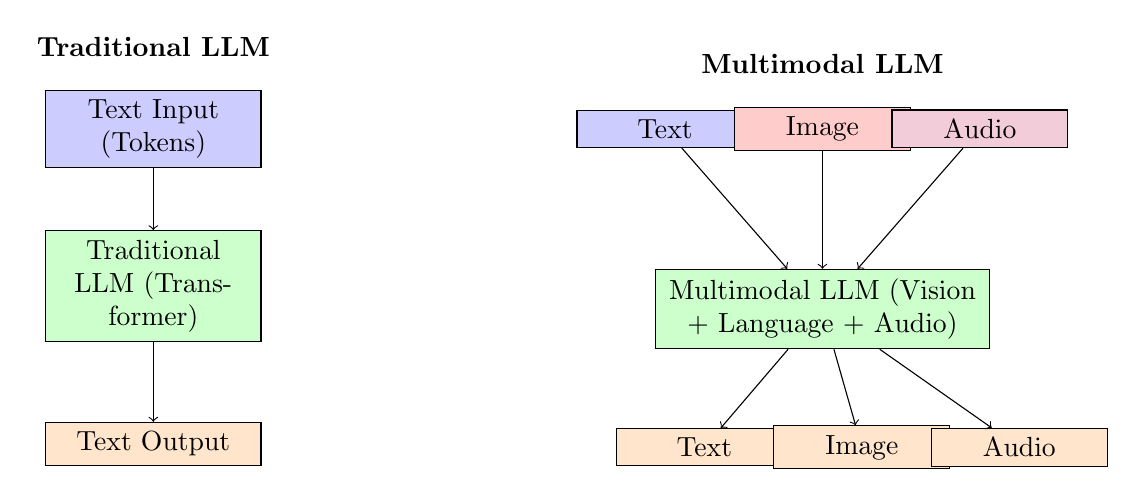
\begin{tikzpicture}[node distance=2cm, auto]
        % Traditional LLM
        \node[draw, rectangle, fill=blue!20, text width=2.5cm, align=center] (input1) {Text Input (Tokens)};
        \node[draw, rectangle, fill=green!20, text width=2.5cm, align=center, below of=input1] (llm) {Traditional LLM (Transformer)};
        \node[draw, rectangle, fill=orange!20, text width=2.5cm, align=center, below of=llm] (output1) {Text Output};
        
        % Arrows for Traditional LLM
        \draw[->] (input1) -- (llm);
        \draw[->] (llm) -- (output1);
        
        % MLLM
        \node[draw, rectangle, fill=blue!20, text width=2cm, align=center, right=4cm of input1] (text) {Text};
        \node[draw, rectangle, fill=red!20, text width=2cm, align=center, right of=text] (image) {Image};
        \node[draw, rectangle, fill=purple!20, text width=2cm, align=center, right of=image] (audio) {Audio};
        
        \node[draw, rectangle, fill=green!20, text width=4cm, align=center, below=1.5cm of image] (mllm) {Multimodal LLM (Vision + Language + Audio)};
        
        \node[draw, rectangle, fill=orange!20, text width=2cm, align=center, below=1cm of mllm, xshift=-1.5cm] (textout) {Text};
        \node[draw, rectangle, fill=orange!20, text width=2cm, align=center, right of=textout] (imageout) {Image};
        \node[draw, rectangle, fill=orange!20, text width=2cm, align=center, right of=imageout] (audioout) {Audio};
        
        % Arrows for MLLM
        \draw[->] (text) -- (mllm);
        \draw[->] (image) -- (mllm);
        \draw[->] (audio) -- (mllm);
        \draw[->] (mllm) -- (textout);
        \draw[->] (mllm) -- (imageout);
        \draw[->] (mllm) -- (audioout);
        
        % Labels
        \node[above=0.3cm of input1, font=\bfseries] {Traditional LLM};
        \node[above=0.3cm of image, font=\bfseries] {Multimodal LLM};
    \end{tikzpicture}
    \caption{Architectural comparison between traditional LLMs and MLLMs showing modality integration}
    \label{fig:llm_mllm_arch_niu}
\end{figure}

\textbf{Architectural and Processing Differences}

Traditional LLMs like GPT-3 and BERT process only text-based inputs through transformer architectures, excelling at natural language tasks within the textual domain. MLLMs integrate multiple modalities (vision, text, audio) using: (1) modality-specific encoders, (2) cross-modal alignment mechanisms, and (3) language model decoders, enabling simultaneous understanding across different modalities.

\textbf{Training and Applications}

Traditional LLMs use self-supervised learning on text corpora with next-token prediction, limiting understanding to linguistic patterns. MLLMs require multi-stage training on multimodal datasets (image-text pairs, video-text combinations), significantly increasing computational requirements.

While traditional LLMs excel in text-centric applications (translation, code completion) but cannot process visual information, MLLMs expand to visual question answering, image captioning, and multimodal dialogue systems. However, this versatility comes with increased complexity and potential performance trade-offs in pure text tasks.

\subsubsection{Response by Wu Zining}
% 吴子宁的回答

\begin{figure}[H]
    \centering
    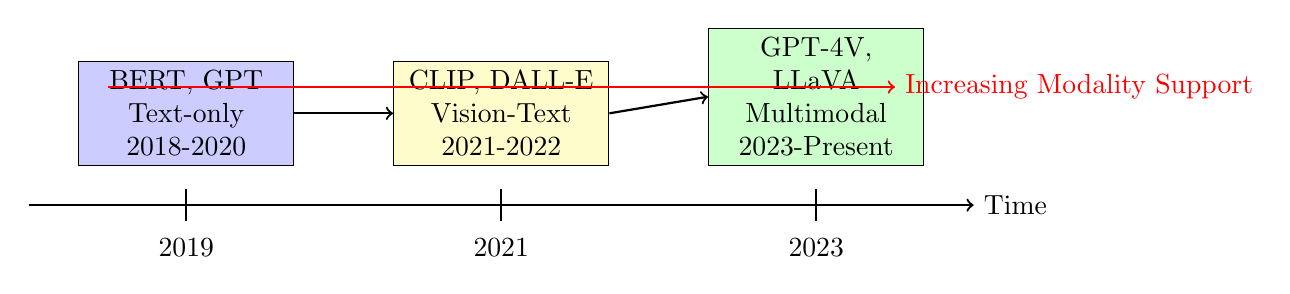
\begin{tikzpicture}[node distance=3cm]
        % Timeline
        \draw[thick, ->] (0,0) -- (12,0) node[right] {Time};
        
        % Traditional LLMs era
        \node[draw, rectangle, fill=blue!20, text width=2.5cm, align=center, above=0.5cm] at (2,0) (bert) {BERT, GPT Text-only 2018-2020};
        \draw[thick] (2,-0.2) -- (2,0.2);
        
        % Transition period
        \node[draw, rectangle, fill=yellow!20, text width=2.5cm, align=center, above=0.5cm] at (6,0) (clip) {CLIP, DALL-E Vision-Text 2021-2022};
        \draw[thick] (6,-0.2) -- (6,0.2);
        
        % MLLM era
        \node[draw, rectangle, fill=green!20, text width=2.5cm, align=center, above=0.5cm] at (10,0) (gpt4v) {GPT-4V, LLaVA Multimodal 2023-Present};
        \draw[thick] (10,-0.2) -- (10,0.2);
        
        % Arrows showing evolution
        \draw[thick, ->] (bert.east) -- (clip.west);
        \draw[thick, ->] (clip.east) -- (gpt4v.west);
        
        % Labels
        \node[below=0.3cm] at (2,0) {2019};
        \node[below=0.3cm] at (6,0) {2021};
        \node[below=0.3cm] at (10,0) {2023};
        
        % Capability arrows
        \draw[thick, red, ->] (1,1.5) -- (11,1.5) node[right] {Increasing Modality Support};
    \end{tikzpicture}
    \caption{Evolution timeline from traditional LLMs to multimodal systems}
    \label{fig:mllm_evolution_wu}
\end{figure}

\textbf{Architectural Evolution: Single to Multiple Modalities}

The evolution from traditional LLMs to MLLMs represents a paradigm shift from single-modality to integrated multimodal understanding. Traditional LLMs operate within textual constraints, processing only tokenized sequences and remaining limited to symbolic language representation.

MLLMs transcend this by incorporating vision encoders, audio processors, and cross-modal components. Typical MLLM architecture features specialized encoders (e.g., Vision Transformer) that convert multimodal inputs into feature representations, then project these features into the language model's embedding space.

\textbf{Processing and Training Differences}

Traditional LLMs employ straightforward tokenization and next-token prediction on text corpora. MLLMs require heterogeneous representation learning, processing different modalities through specialized encoders before fusion in shared representational space. Training involves: (1) vision-language pre-training, (2) multimodal instruction tuning, and (3) task-specific fine-tuning, significantly increasing computational costs and requiring specialized expertise in cross-modal alignment.

\subsubsection{Response by Zhao Jinqiu}
% 赵金秋的回答

\begin{figure}[H]
    \centering
    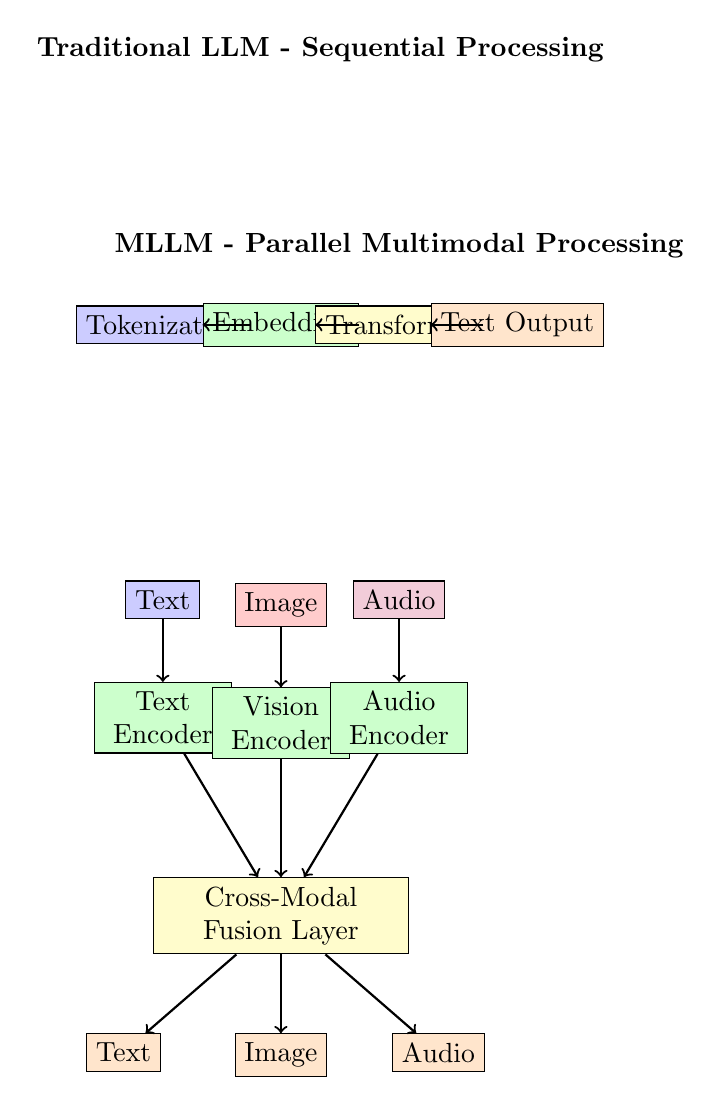
\begin{tikzpicture}[node distance=1.5cm]
        % Sequential Processing (Traditional LLM)
        \node[font=\bfseries] at (2, 3.5) {Traditional LLM - Sequential Processing};
        \node[draw, rectangle, fill=blue!20] (tok1) {Tokenization};
        \node[draw, rectangle, fill=green!20, right of=tok1] (emb1) {Embedding};
        \node[draw, rectangle, fill=yellow!20, right of=emb1] (trans1) {Transformer};
        \node[draw, rectangle, fill=orange!20, right of=trans1] (out1) {Text Output};
        
        \draw[thick, ->] (tok1) -- (emb1);
        \draw[thick, ->] (emb1) -- (trans1);
        \draw[thick, ->] (trans1) -- (out1);
        
        % Parallel Processing (MLLM)
        \node[font=\bfseries] at (3, 1) {MLLM - Parallel Multimodal Processing};
        
        % Input modalities
        \node[draw, rectangle, fill=blue!20, below=3cm of tok1] (text2) {Text};
        \node[draw, rectangle, fill=red!20, below=3cm of emb1] (img2) {Image};
        \node[draw, rectangle, fill=purple!20, below=3cm of trans1] (aud2) {Audio};
        
        % Encoders
        \node[draw, rectangle, fill=green!20, below of=text2, text width=1.5cm, align=center] (textenc) {Text Encoder};
        \node[draw, rectangle, fill=green!20, below of=img2, text width=1.5cm, align=center] (imgenc) {Vision Encoder};
        \node[draw, rectangle, fill=green!20, below of=aud2, text width=1.5cm, align=center] (audenc) {Audio Encoder};
        
        % Fusion layer
        \node[draw, rectangle, fill=yellow!20, below=1.5cm of imgenc, text width=3cm, align=center] (fusion) {Cross-Modal Fusion Layer};
        
        % Outputs
        \node[draw, rectangle, fill=orange!20, below=1cm of fusion, xshift=-2cm] (textout2) {Text};
        \node[draw, rectangle, fill=orange!20, below=1cm of fusion] (imgout2) {Image};
        \node[draw, rectangle, fill=orange!20, below=1cm of fusion, xshift=2cm] (audout2) {Audio};
        
        % Arrows
        \draw[thick, ->] (text2) -- (textenc);
        \draw[thick, ->] (img2) -- (imgenc);
        \draw[thick, ->] (aud2) -- (audenc);
        
        \draw[thick, ->] (textenc) -- (fusion);
        \draw[thick, ->] (imgenc) -- (fusion);
        \draw[thick, ->] (audenc) -- (fusion);
        
        \draw[thick, ->] (fusion) -- (textout2);
        \draw[thick, ->] (fusion) -- (imgout2);
        \draw[thick, ->] (fusion) -- (audout2);
    \end{tikzpicture}
    \caption{Comparison of sequential processing in traditional LLMs vs. parallel multimodal processing in MLLMs}
    \label{fig:processing_comparison_zhao}
\end{figure}

\textbf{Processing Philosophy: Unimodal vs. Multimodal Intelligence}

Traditional LLMs embody a text-centric paradigm where all capabilities are mediated through linguistic representations. Models like GPT-3.5 process information exclusively through tokenized text sequences, excelling in language comprehension within textual confines.

MLLMs represent a shift toward embodied intelligence, integrating multiple sensory modalities similar to human cognitive processes. Models like GPT-4V and LLaVA simultaneously process text, images, and audio, enabling richer contextual understanding.

\textbf{Technical Architecture and Applications}

Traditional LLMs employ sequential processing with linear pipeline: tokenization → embedding → transformer layers → output generation. MLLMs implement parallel modality processing with: (1) modality-specific encoders, (2) cross-modal attention mechanisms, (3) alignment modules, and (4) unified decoders.

Traditional LLMs use single-task optimization with established language modeling objectives. MLLMs face complex multi-objective optimization, balancing learning across modalities. Applications expand from text-centric tasks (summarization, code generation) to cross-modal capabilities (visual question answering, image captioning, multimodal dialogue systems).

\subsection{LLaVA Model Performance Evaluation}
% LLaVA模型性能评估

To demonstrate practical MLLM capabilities, we deployed the \texttt{llava-interleave-qwen-0.5b-hf} model from the LLaVA Model Zoo and evaluated its performance across two representative multimodal tasks: image captioning and visual question answering. This compact 0.5B parameter variant provides an efficient balance between computational requirements and multimodal understanding capabilities.
% 为了展示实用的MLLM能力,我们部署了来自LLaVA模型库的llava-interleave-qwen-0.5b-hf模型,并在两个代表性的多模态任务上评估其性能:图像描述和视觉问答。

\subsubsection{Model Architecture and Deployment}
% 模型架构和部署

The LLaVA-Interleave-Qwen-0.5B model integrates a vision transformer encoder with the Qwen language model backbone, enabling seamless processing of interleaved image-text sequences. The deployment utilized the Hugging Face Transformers framework with specialized configuration for multimodal inference, supporting both image captioning and conversational visual analysis.
% LLaVA-Interleave-Qwen-0.5B模型集成了视觉transformer编码器与Qwen语言模型主干,支持交错图像-文本序列的无缝处理。

\subsubsection{Image Captioning Performance}
% 图像描述性能

We evaluated the model's image captioning capabilities using an equestrian scene featuring a rider on horseback (Figure~\ref{fig:knight_horse_image}). The model was tasked with generating detailed descriptions that capture both visual elements and contextual understanding.
% 我们使用一个骑士骑马的马术场景评估了模型的图像描述能力。

\begin{figure}[H]
    \centering
    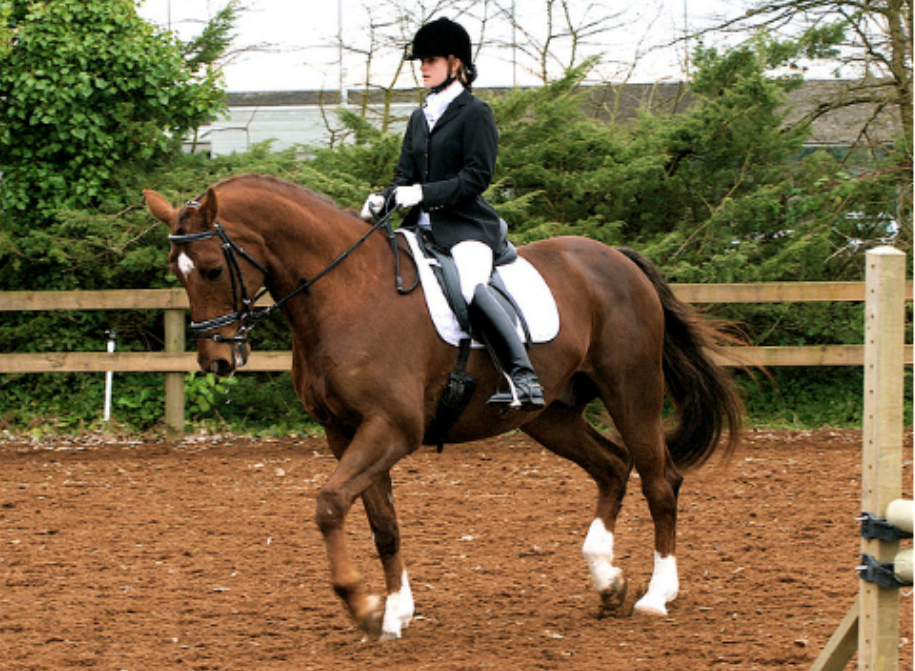
\includegraphics[width=0.8\textwidth]{Figures/knight with horse.png}
    \caption{Equestrian scene used for image captioning evaluation: rider in formal attire on a brown horse in an outdoor arena}
    % 用于图像描述评估的马术场景:穿着正装的骑手在户外竞技场骑棕色马匹
    \label{fig:knight_horse_image}
\end{figure}

The model demonstrated strong visual comprehension, accurately identifying key elements including the rider's formal black riding attire, the horse's brown coat with white markings, the outdoor arena setting with wooden fencing, and the overall equestrian context. The generated description exhibited both detailed visual recognition and appropriate contextual interpretation, showcasing the model's ability to process complex visual scenes and generate coherent natural language descriptions.
% 模型展现了强大的视觉理解能力,准确识别了包括骑手的黑色正装、马匹的棕色毛色和白色斑纹、带木栅栏的户外竞技场环境等关键元素。

\subsubsection{Interactive Visual Question Answering}
% 交互式视觉问答

Beyond static captioning, we conducted interactive dialogue sessions to evaluate the model's visual question answering capabilities and conversational coherence. Figure~\ref{fig:llava_conversation} demonstrates a multi-turn conversation where the model successfully engaged in contextual dialogue about the image content.
% 除了静态描述,我们进行了交互式对话会话来评估模型的视觉问答能力和对话连贯性。

\begin{figure}[H]
    \centering
    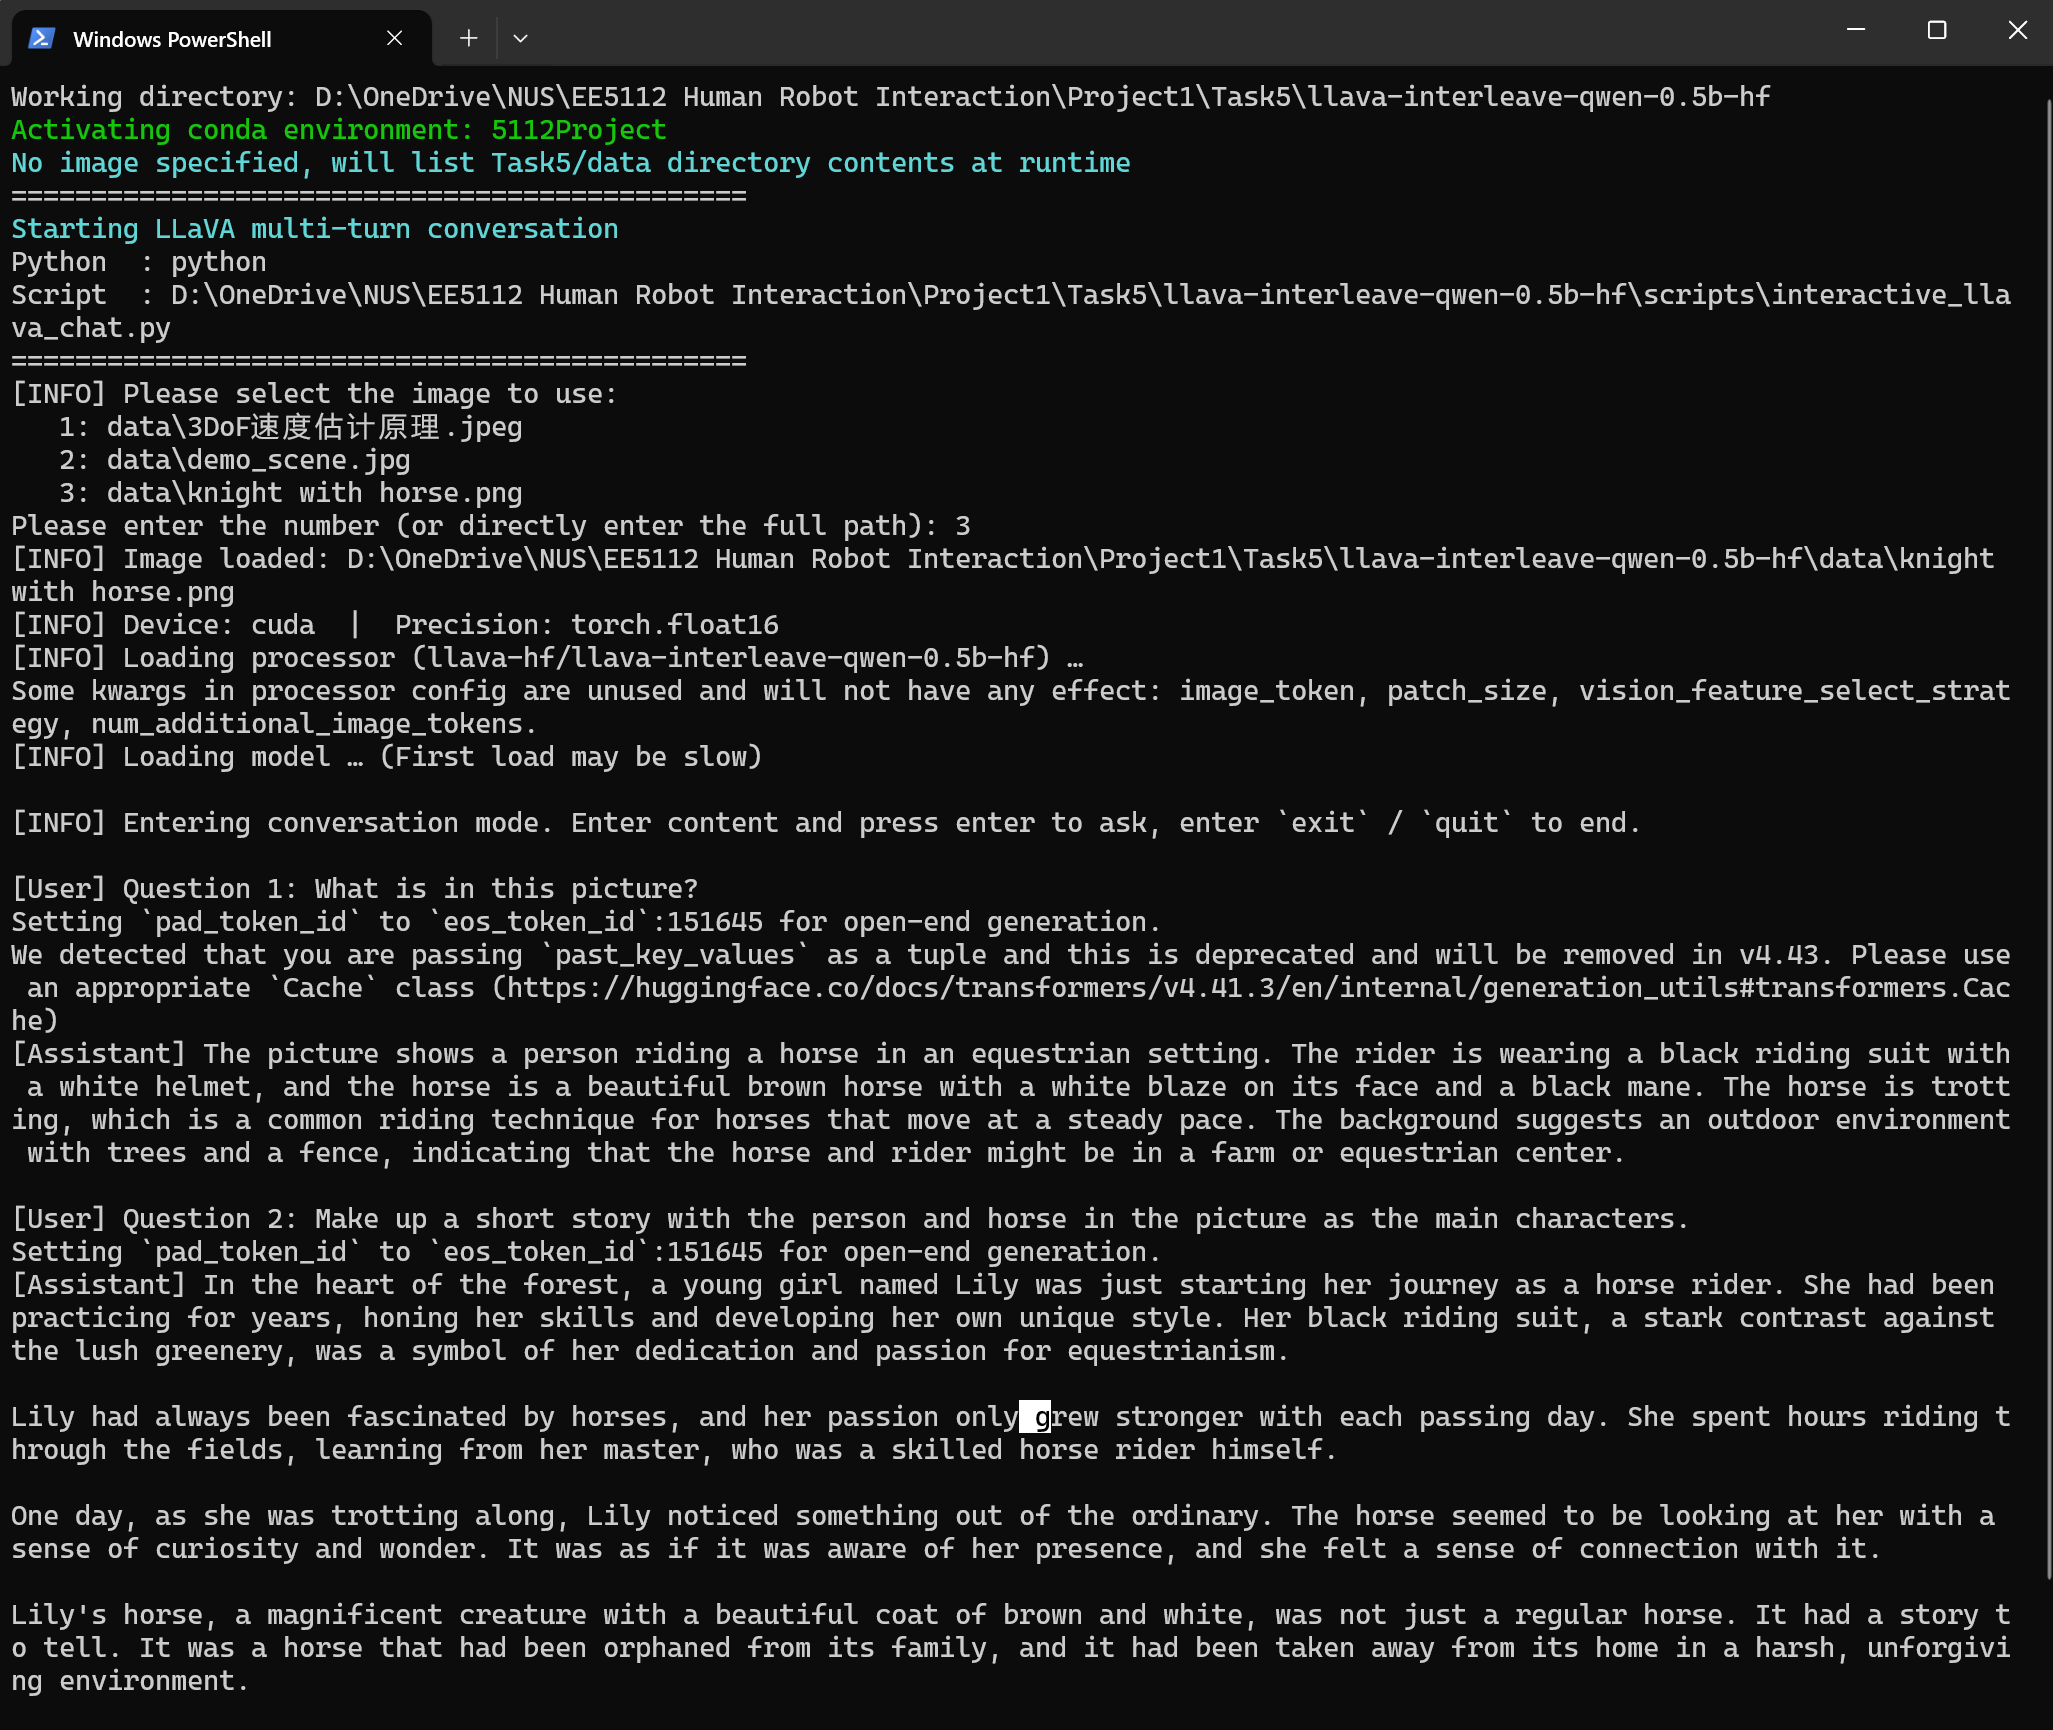
\includegraphics[width=0.95\textwidth]{Figures/多模态对话.png}
    \caption{Interactive dialogue session with LLaVA model showing multi-turn visual question answering and story generation capabilities}
    % 与LLaVA模型的交互对话会话,展示多轮视觉问答和故事生成能力
    \label{fig:llava_conversation}
\end{figure}

The conversation transcript reveals several key capabilities:
% 对话记录显示了几个关键能力:

\begin{enumerate}
    \item \textbf{Detailed Visual Analysis}: The model provided comprehensive scene description, identifying the person's attire (black riding suit with helmet), horse characteristics (brown with white blaze and mane), and environmental context (farm or equestrian center with trees and fence).
    % 详细的视觉分析:模型提供了全面的场景描述
    
    \item \textbf{Creative Narrative Generation}: When prompted to create a story, the model generated a coherent narrative about "Lily," demonstrating its ability to synthesize visual information with creative storytelling, including character development and emotional context.
    % 创意叙事生成:当被要求创作故事时,模型生成了关于"Lily"的连贯叙事
    
    \item \textbf{Contextual Dialogue Maintenance}: The model maintained conversational context across multiple turns, appropriately referencing previous interactions and building upon established narrative elements.
    % 上下文对话维护:模型在多轮对话中保持了对话上下文
\end{enumerate}

\subsubsection{Performance Assessment and Limitations}
% 性能评估和局限性

The LLaVA-Interleave-Qwen-0.5B model demonstrates robust multimodal capabilities despite its compact size. Strengths include accurate object recognition, spatial relationship understanding, and coherent text generation. The model successfully bridged visual perception with linguistic expression, generating contextually appropriate responses that demonstrate genuine understanding rather than superficial pattern matching.
% LLaVA-Interleave-Qwen-0.5B模型尽管体积紧凑,但展现了强大的多模态能力。

However, certain limitations emerged during evaluation. The model occasionally exhibited minor factual inconsistencies in fine-grained details and showed some tendency toward verbose responses that could benefit from more concise expression. Additionally, while the creative storytelling capability is impressive, the generated narratives sometimes lack deeper thematic complexity compared to larger models.
% 然而,在评估过程中也出现了某些局限性,如在细粒度细节上偶尔出现轻微的事实不一致。

The successful deployment and evaluation of this MLLM variant demonstrates the practical viability of multimodal systems for real-world applications, providing a foundation for future development in human-robot interaction scenarios where visual understanding and natural language communication must seamlessly integrate.
% 该MLLM变体的成功部署和评估证明了多模态系统在实际应用中的可行性。


\section{Results and Discussion}
% 结果和讨论

% 结果和讨论 - 对项目成果的深入讨论和分析
% Results and discussion - In-depth discussion and analysis of project outcomes

\subsection{System Performance Results}
% 系统性能结果

% 系统性能结果 - 展示系统测试结果
% System performance results - Present system testing results

[Placeholder for system performance results content]
% [系统性能结果内容占位符]

\subsection{Task Achievement Summary}
% 任务完成情况总结

% 任务完成情况总结 - 总结各任务的完成情况
% Task achievement summary - Summary of completion status for each task

[Placeholder for task achievement summary content]
% [任务完成情况总结内容占位符]

\subsection{Lessons Learned}
% 经验教训

% 经验教训 - 从项目中学到的经验
% Lessons learned - Experiences gained from the project

[Placeholder for lessons learned content]
% [经验教训内容占位符]

\section{Individual Contributions}
% 个人贡献

% 个人贡献 - 每个组员的个人贡献说明
% Individual contributions - Individual contribution statements for each group member

\subsection{Member 1: Niu Mu}
% 组员1:牛牧

% 组员1:牛牧 - 个人贡献说明
% Member 1: Niu Mu - Individual contribution statement

[Placeholder for Niu Mu's contributions]
% [牛牧贡献占位符]

\subsection{Member 2: Wu Zining (A0294373W)}
% 组员2:吴子宁

% 组员2:吴子宁 - 个人贡献说明
% Member 2: Wu Zining - Individual contribution statement

[Placeholder for Wu Zining's contributions]
% [吴子宁贡献占位符]

\subsection{Member 3: Zhao Jinqiu}
% 组员3:赵金秋

% 组员3:赵金秋 - 个人贡献说明
% Member 3: Zhao Jinqiu - Individual contribution statement

[Placeholder for Zhao Jinqiu's contributions]
% [赵金秋贡献占位符]

\section{Conclusion}
% 结论

% 结论 - 总结项目成果和贡献
% Conclusion - Summary of project outcomes and contributions

\subsection{Project Objectives Achievement}
% 项目目标达成情况

% 项目目标达成情况 - 总结项目目标的完成情况
% Project objectives achievement - Summary of project objective completion

[Placeholder for project objectives achievement content]
% [项目目标达成情况内容占位符]

\subsection{Future Work}
% 未来工作

% 未来工作 - 可能的改进方向
% Future work - Possible directions for improvement

[Placeholder for future work content]
% [未来工作内容占位符]

\section{References}
% 参考文献

\printbibliography
% 打印参考文献列表

\section{Appendix}
% 附录

% 附录 - 补充材料如代码片段、配置文件等
% Appendix - Supplementary materials such as code snippets, configuration files, etc.

\subsection{Code Documentation}
% 代码文档

% 代码文档 - 主要代码片段的文档
% Code documentation - Documentation of main code snippets

[Placeholder for code documentation]
% [代码文档占位符]

\subsection{Configuration Files}
% 配置文件

% 配置文件 - 系统配置文件
% Configuration files - System configuration files

[Placeholder for configuration files]
% [配置文件占位符]

\subsection{User Manual}
% 用户手册

% 用户手册 - 系统使用说明
% User manual - System usage instructions

[Placeholder for user manual]
% [用户手册占位符]

\end{document}
% 文档结束
